\begin{figure*}[htbp]
\begin{subfigure}{0.48\textwidth}
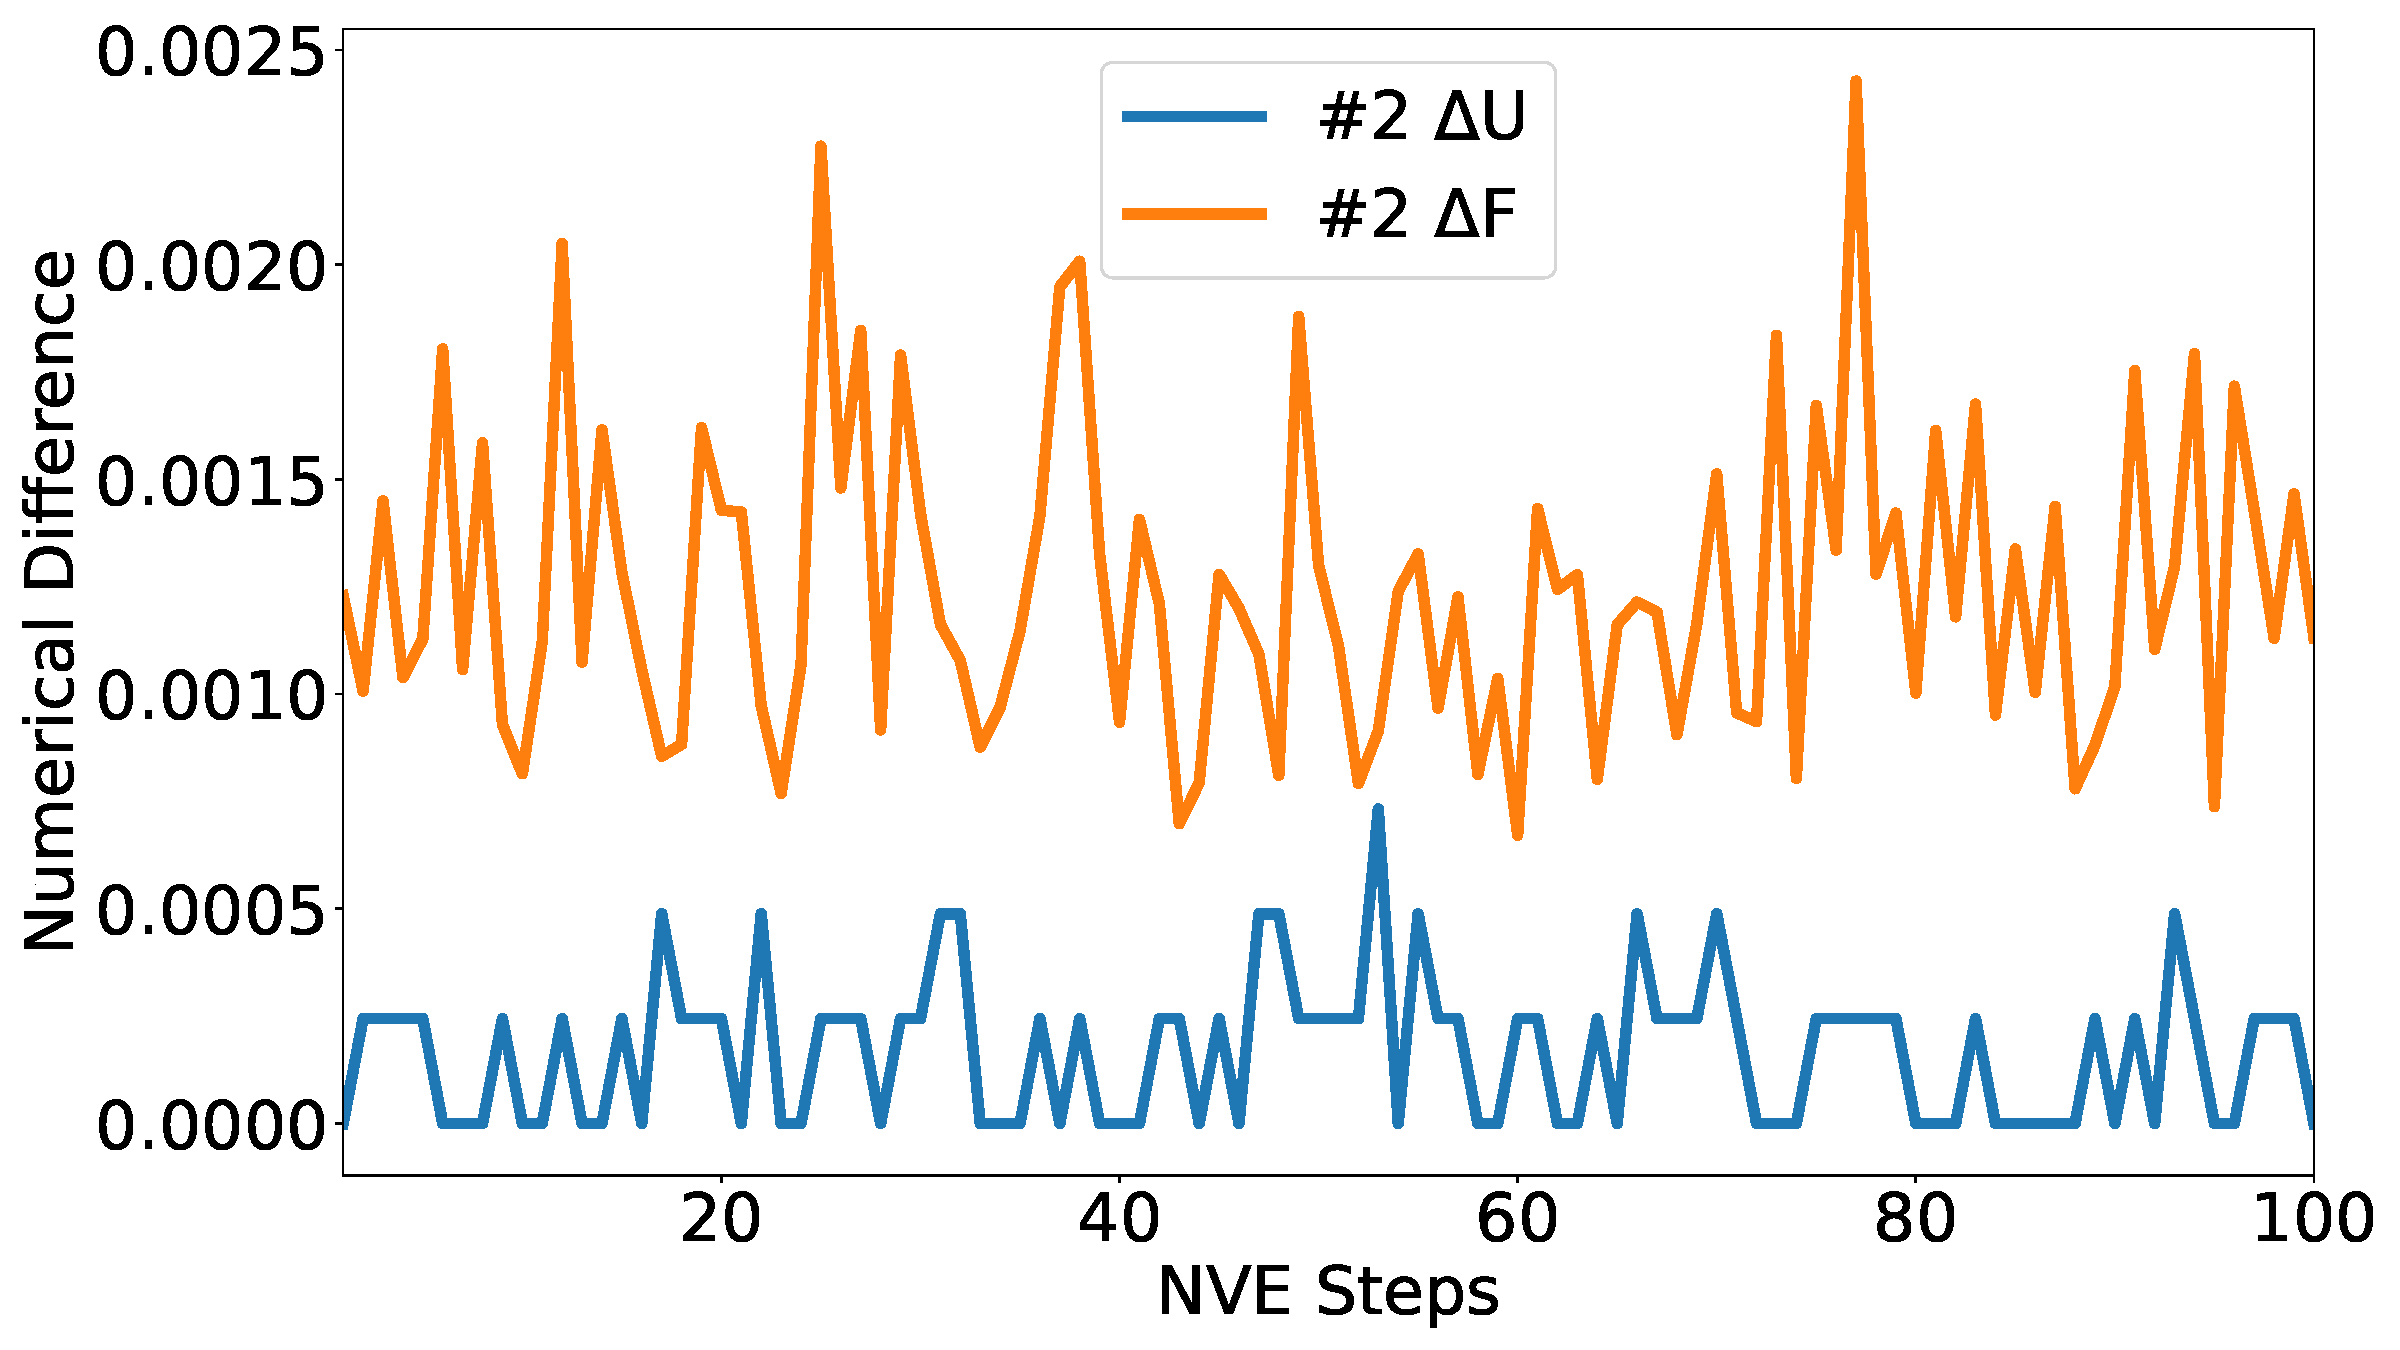
\includegraphics[width=\linewidth]{figs/rerun2.pdf}
\end{subfigure}
\\
\begin{subfigure}{0.48\textwidth}
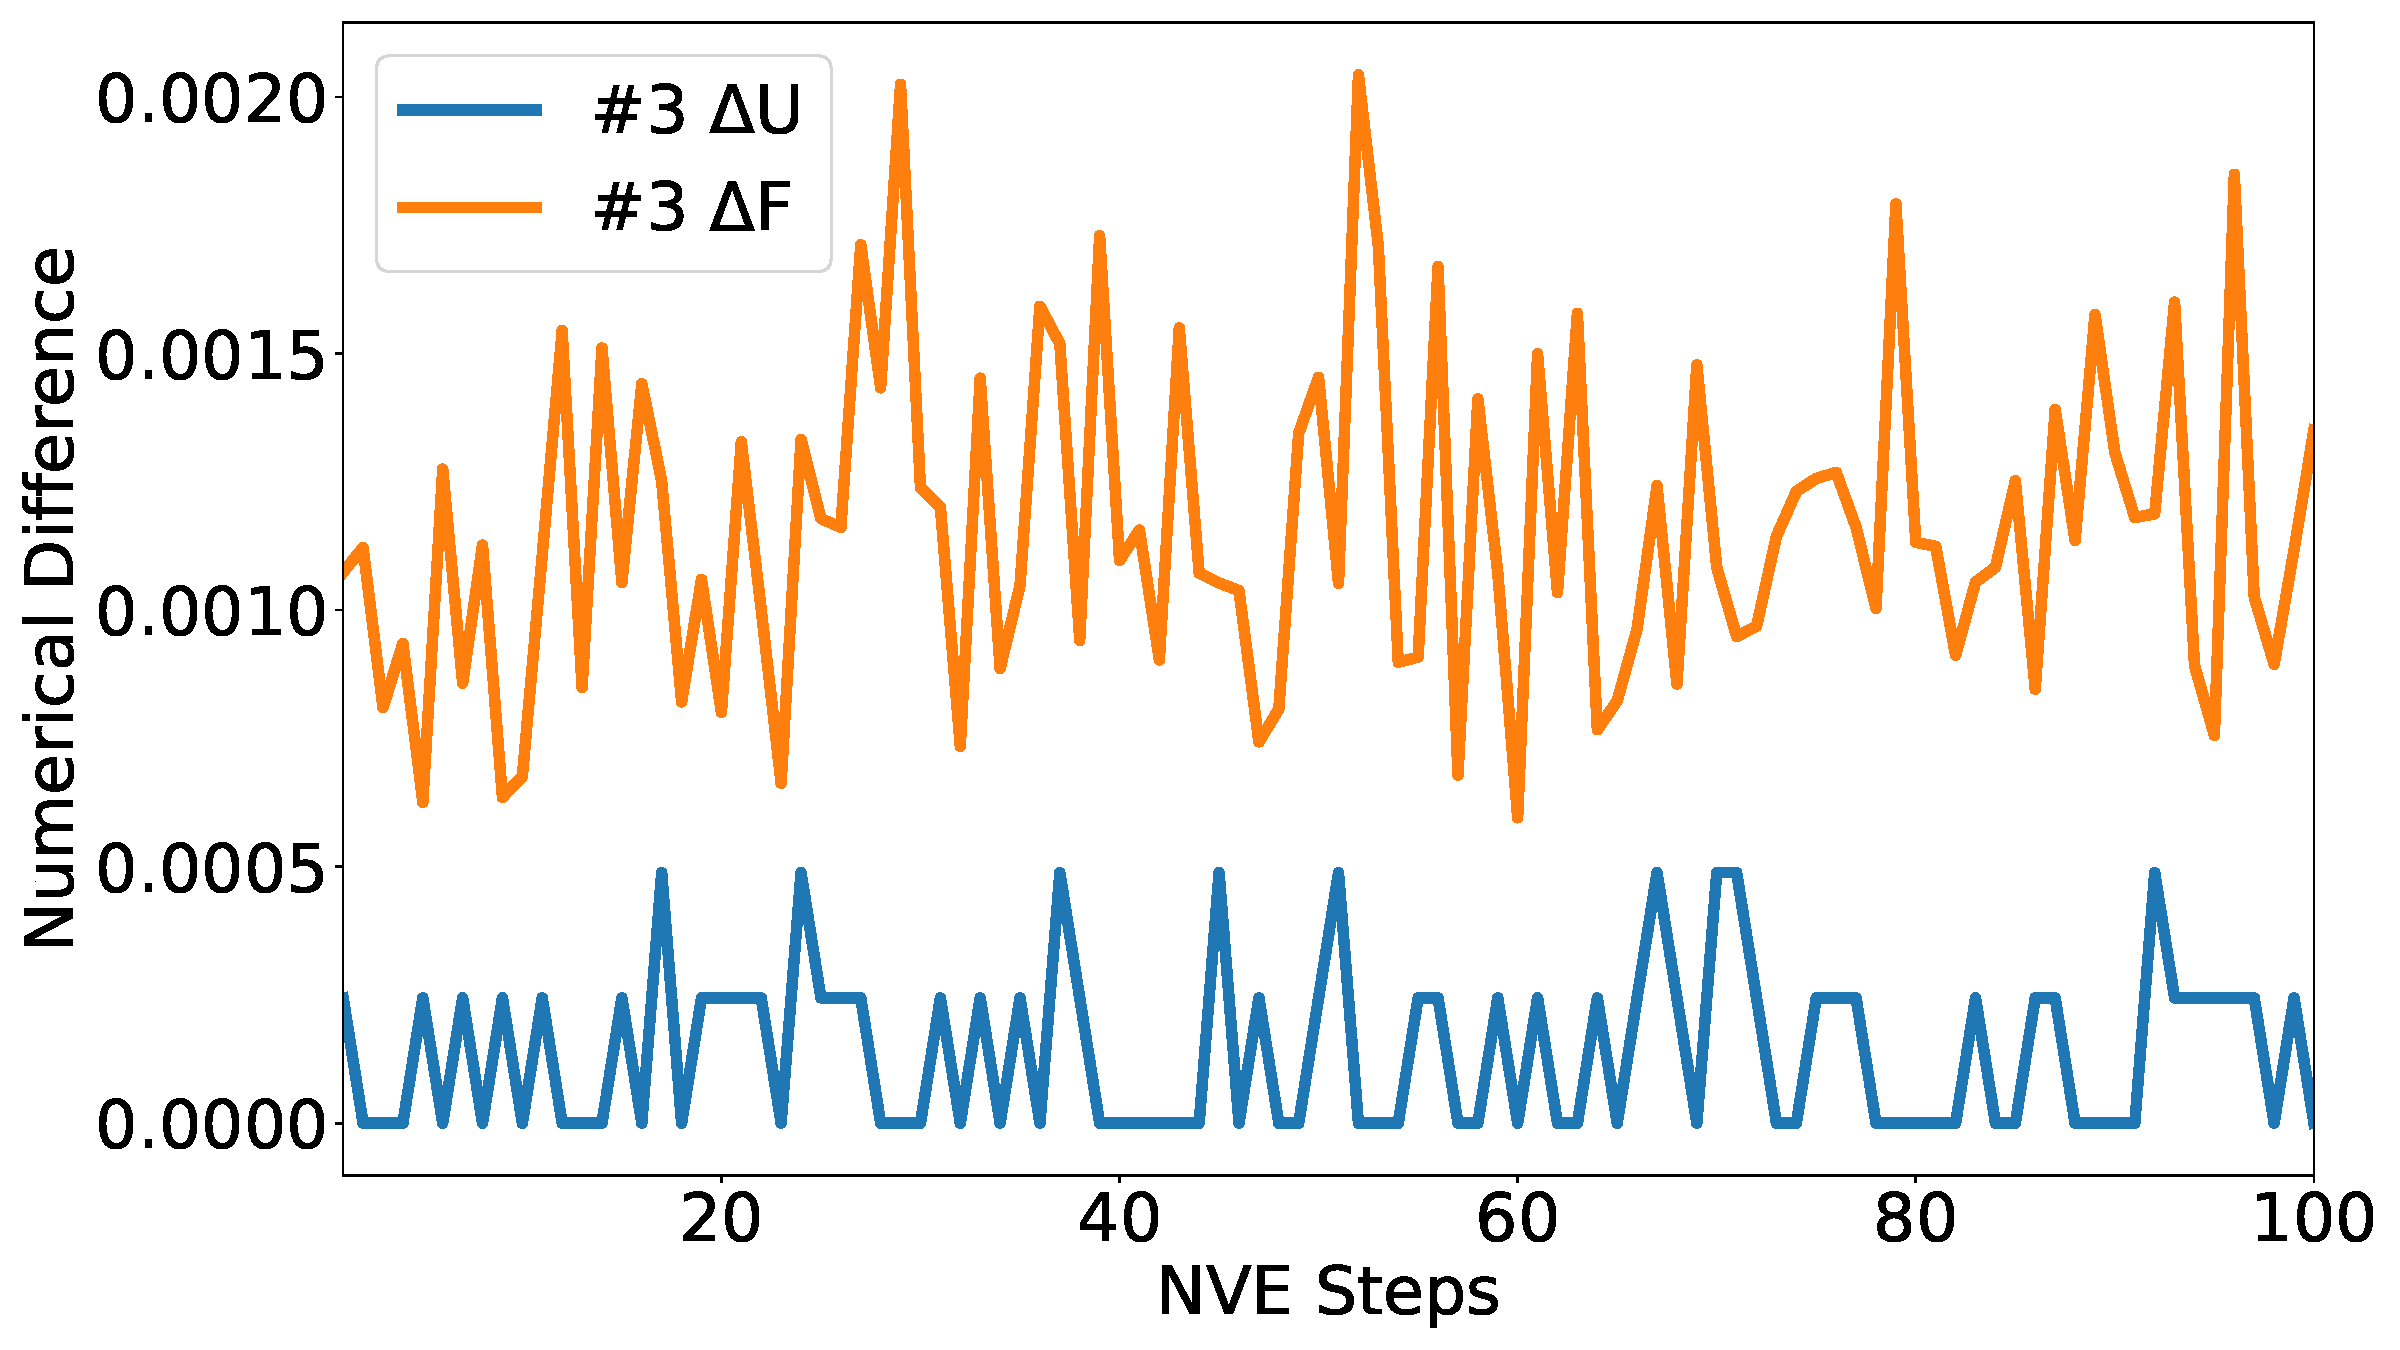
\includegraphics[width=\linewidth]{figs/rerun3.pdf}
\end{subfigure}
\begin{subfigure}{0.48\textwidth}
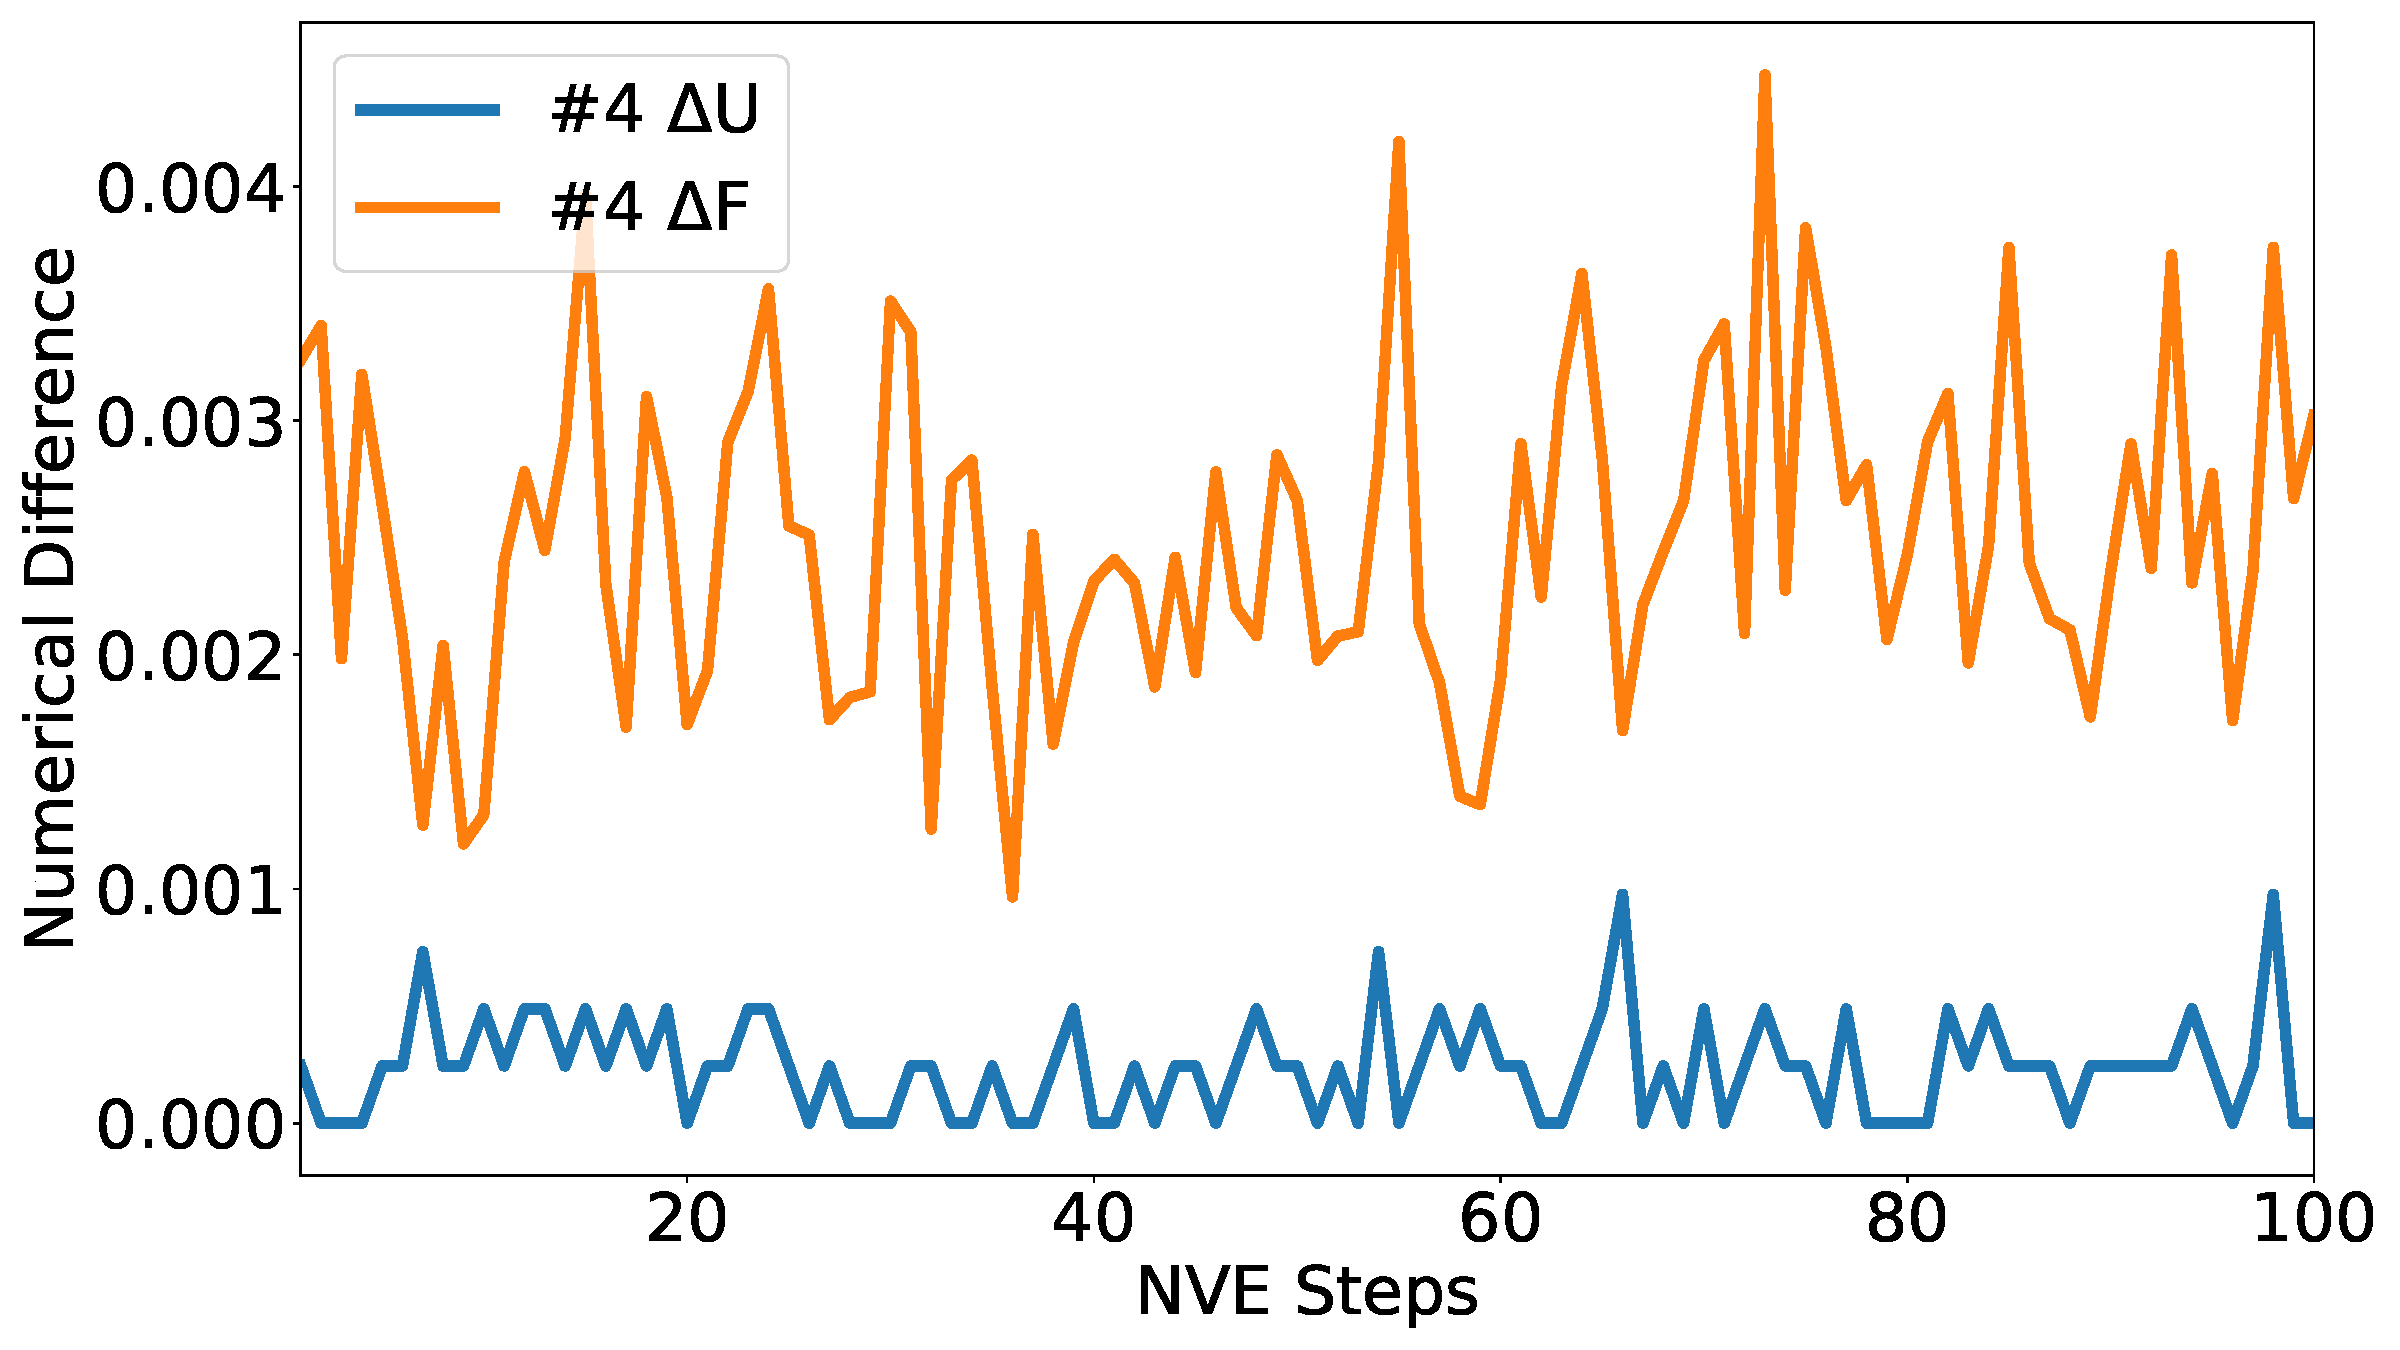
\includegraphics[width=\linewidth]{figs/rerun4.pdf}
\end{subfigure}
\\
\begin{subfigure}{0.48\textwidth}
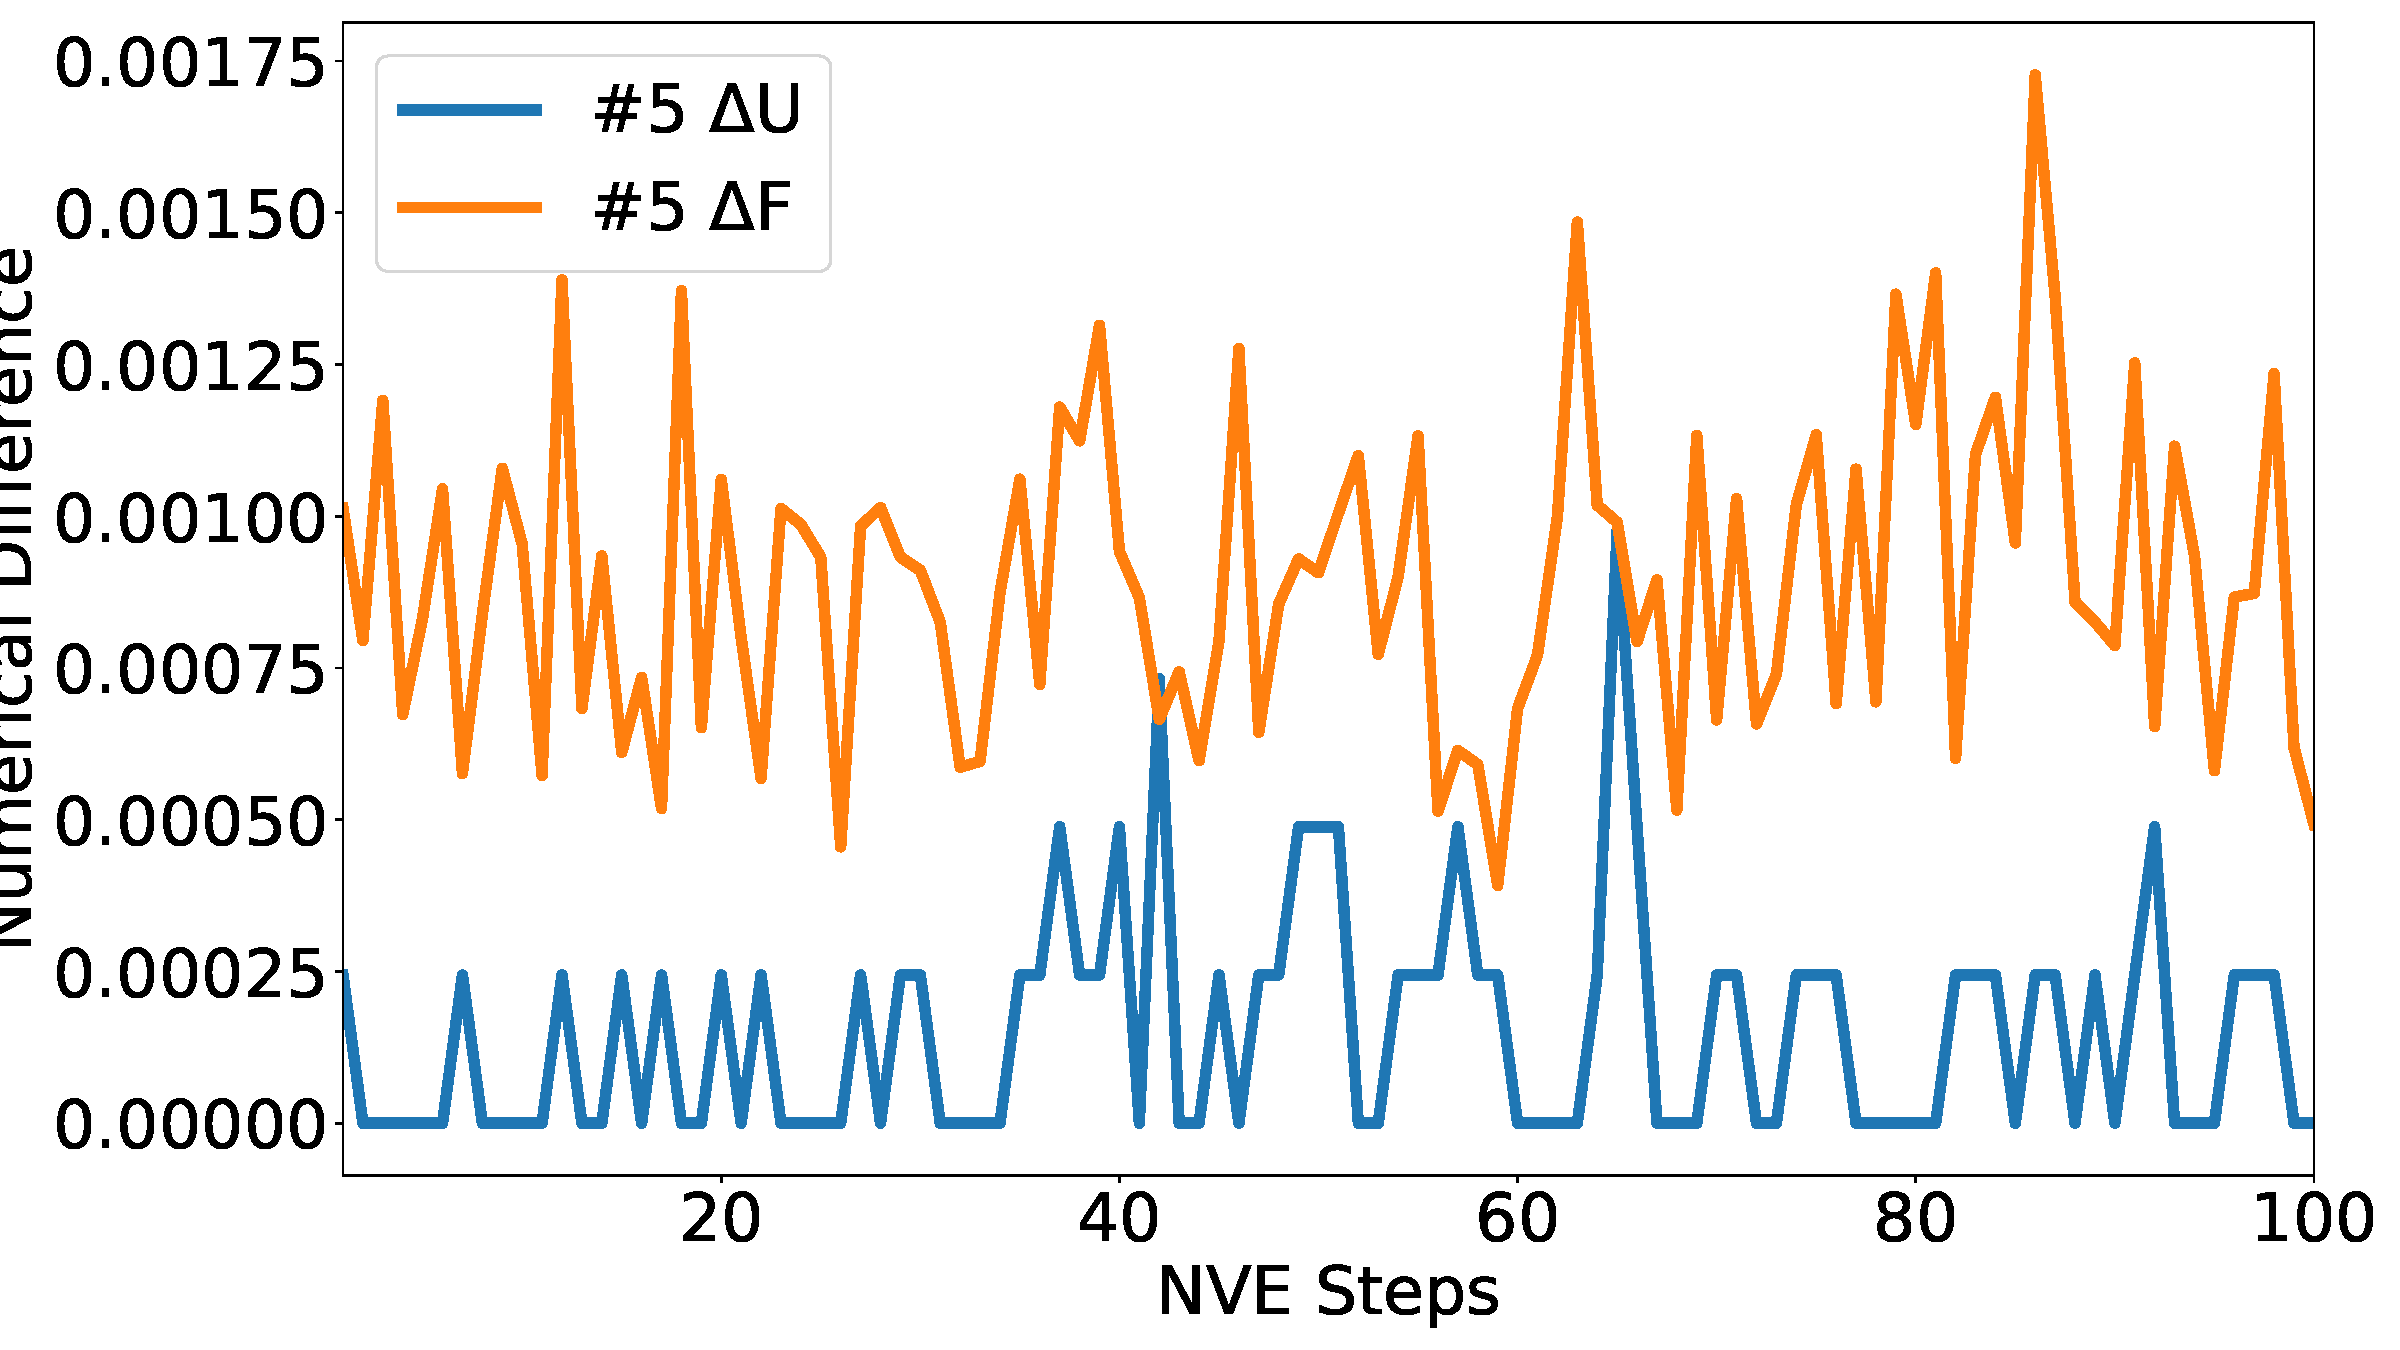
\includegraphics[width=\linewidth]{figs/rerun5.pdf}
\end{subfigure}
\begin{subfigure}{0.48\textwidth}
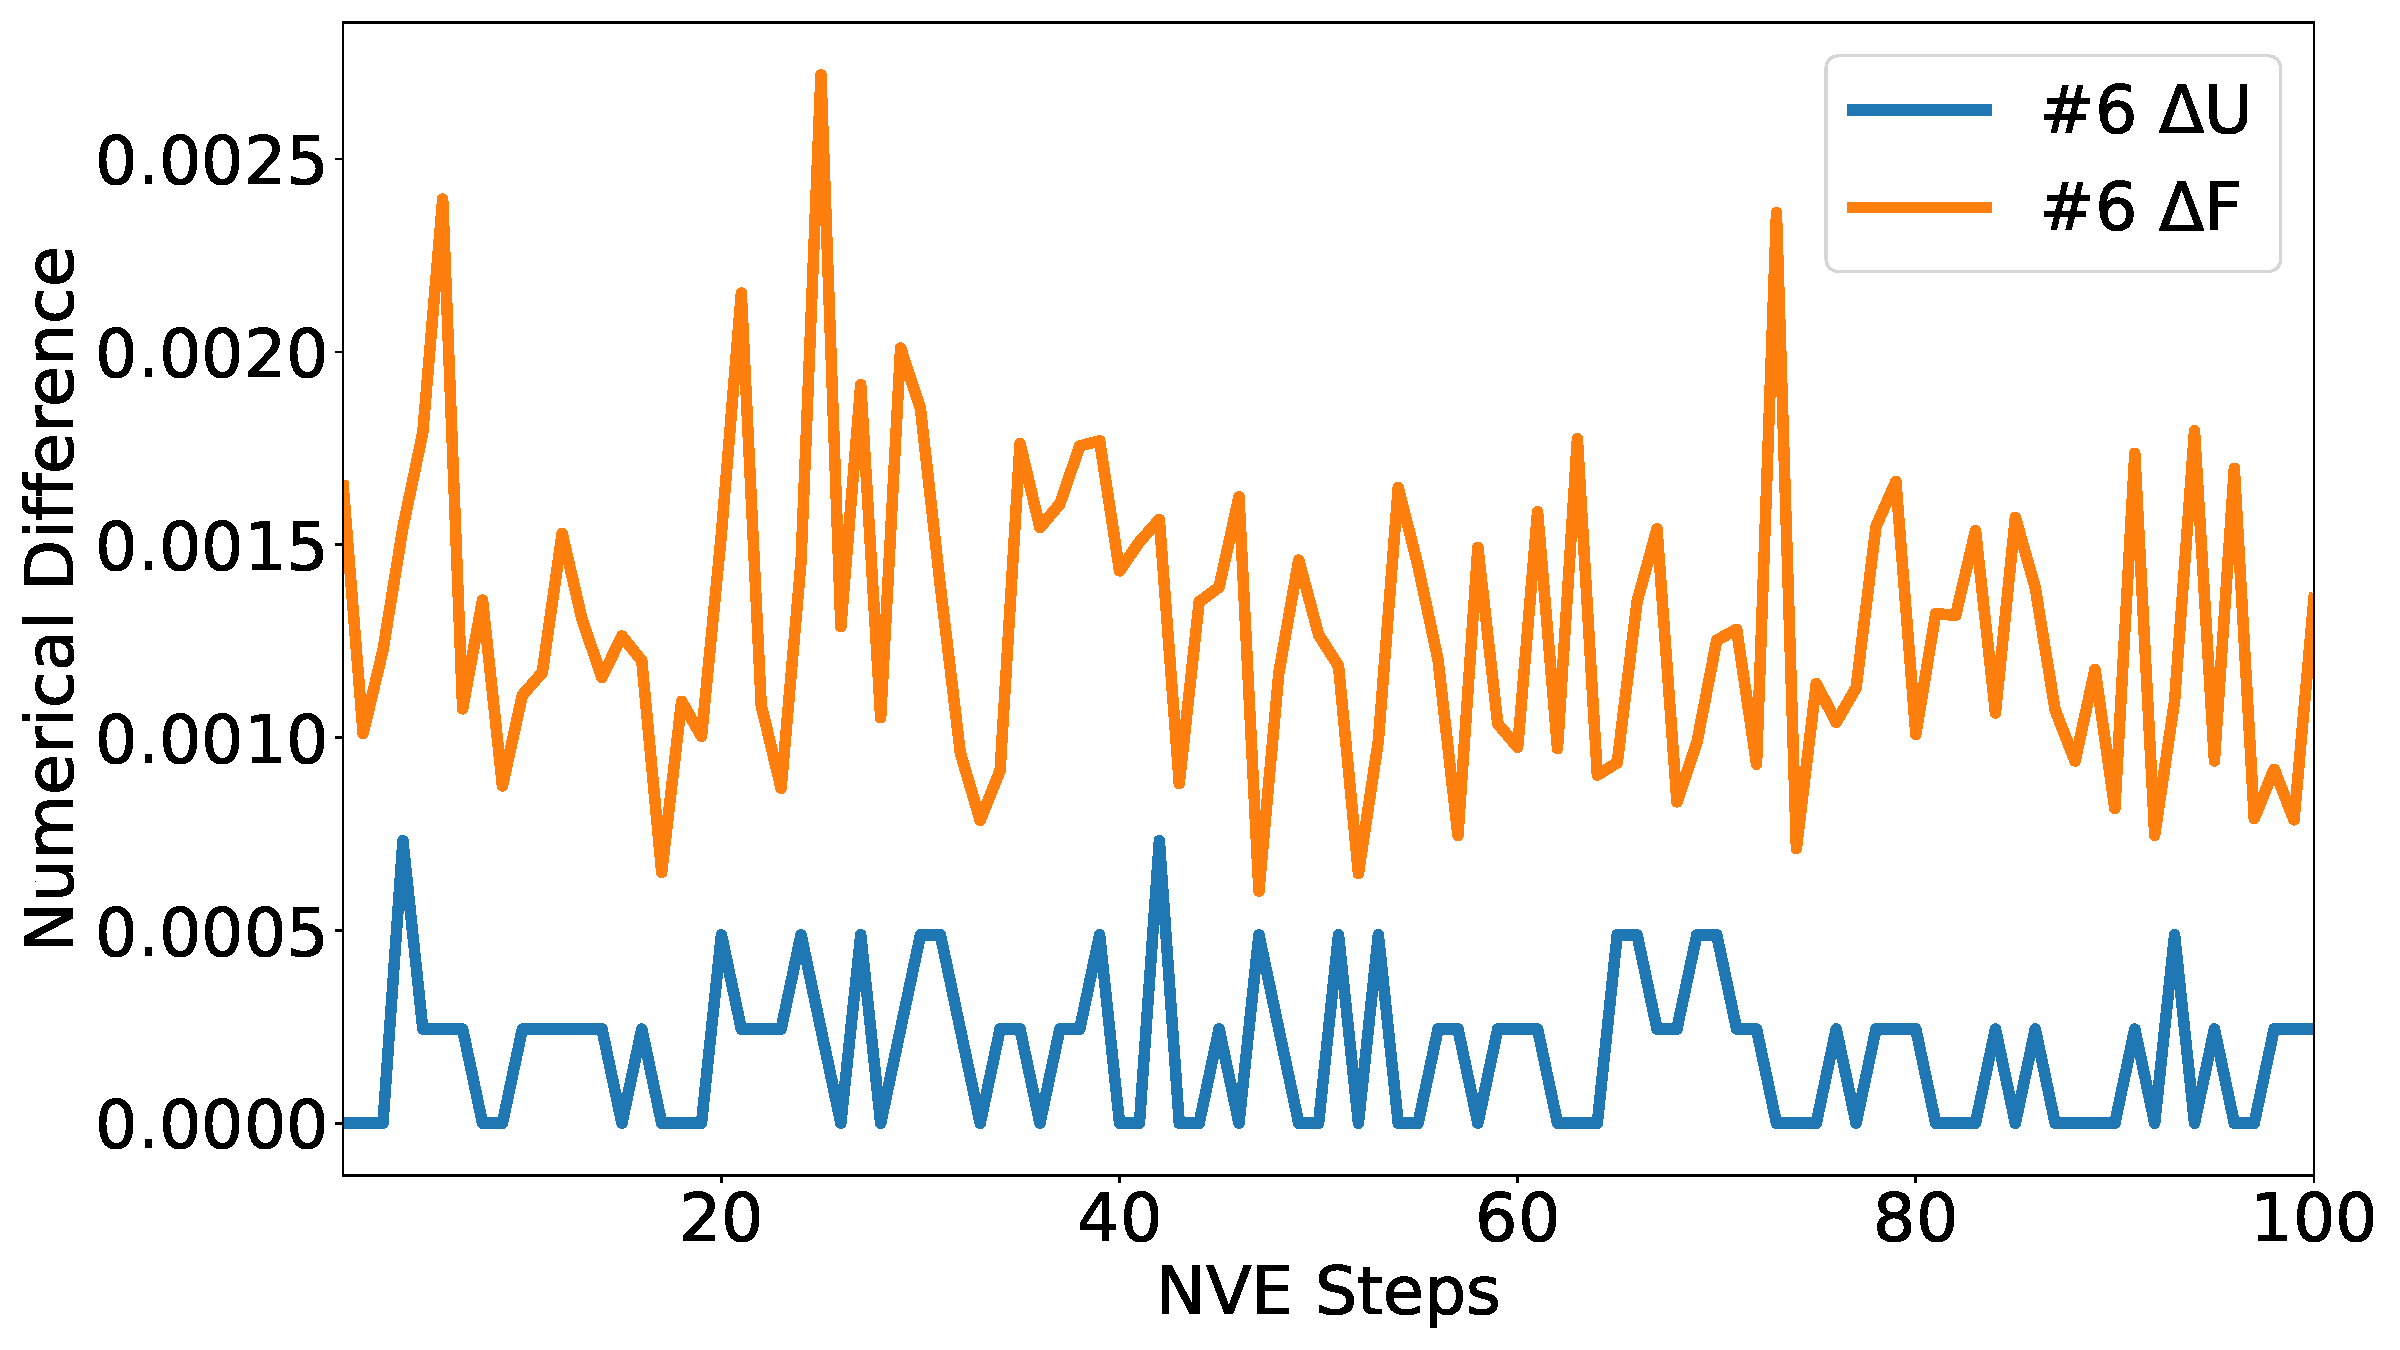
\includegraphics[width=\linewidth]{figs/rerun6.pdf}
\end{subfigure}
\\
\begin{subfigure}{0.48\textwidth}
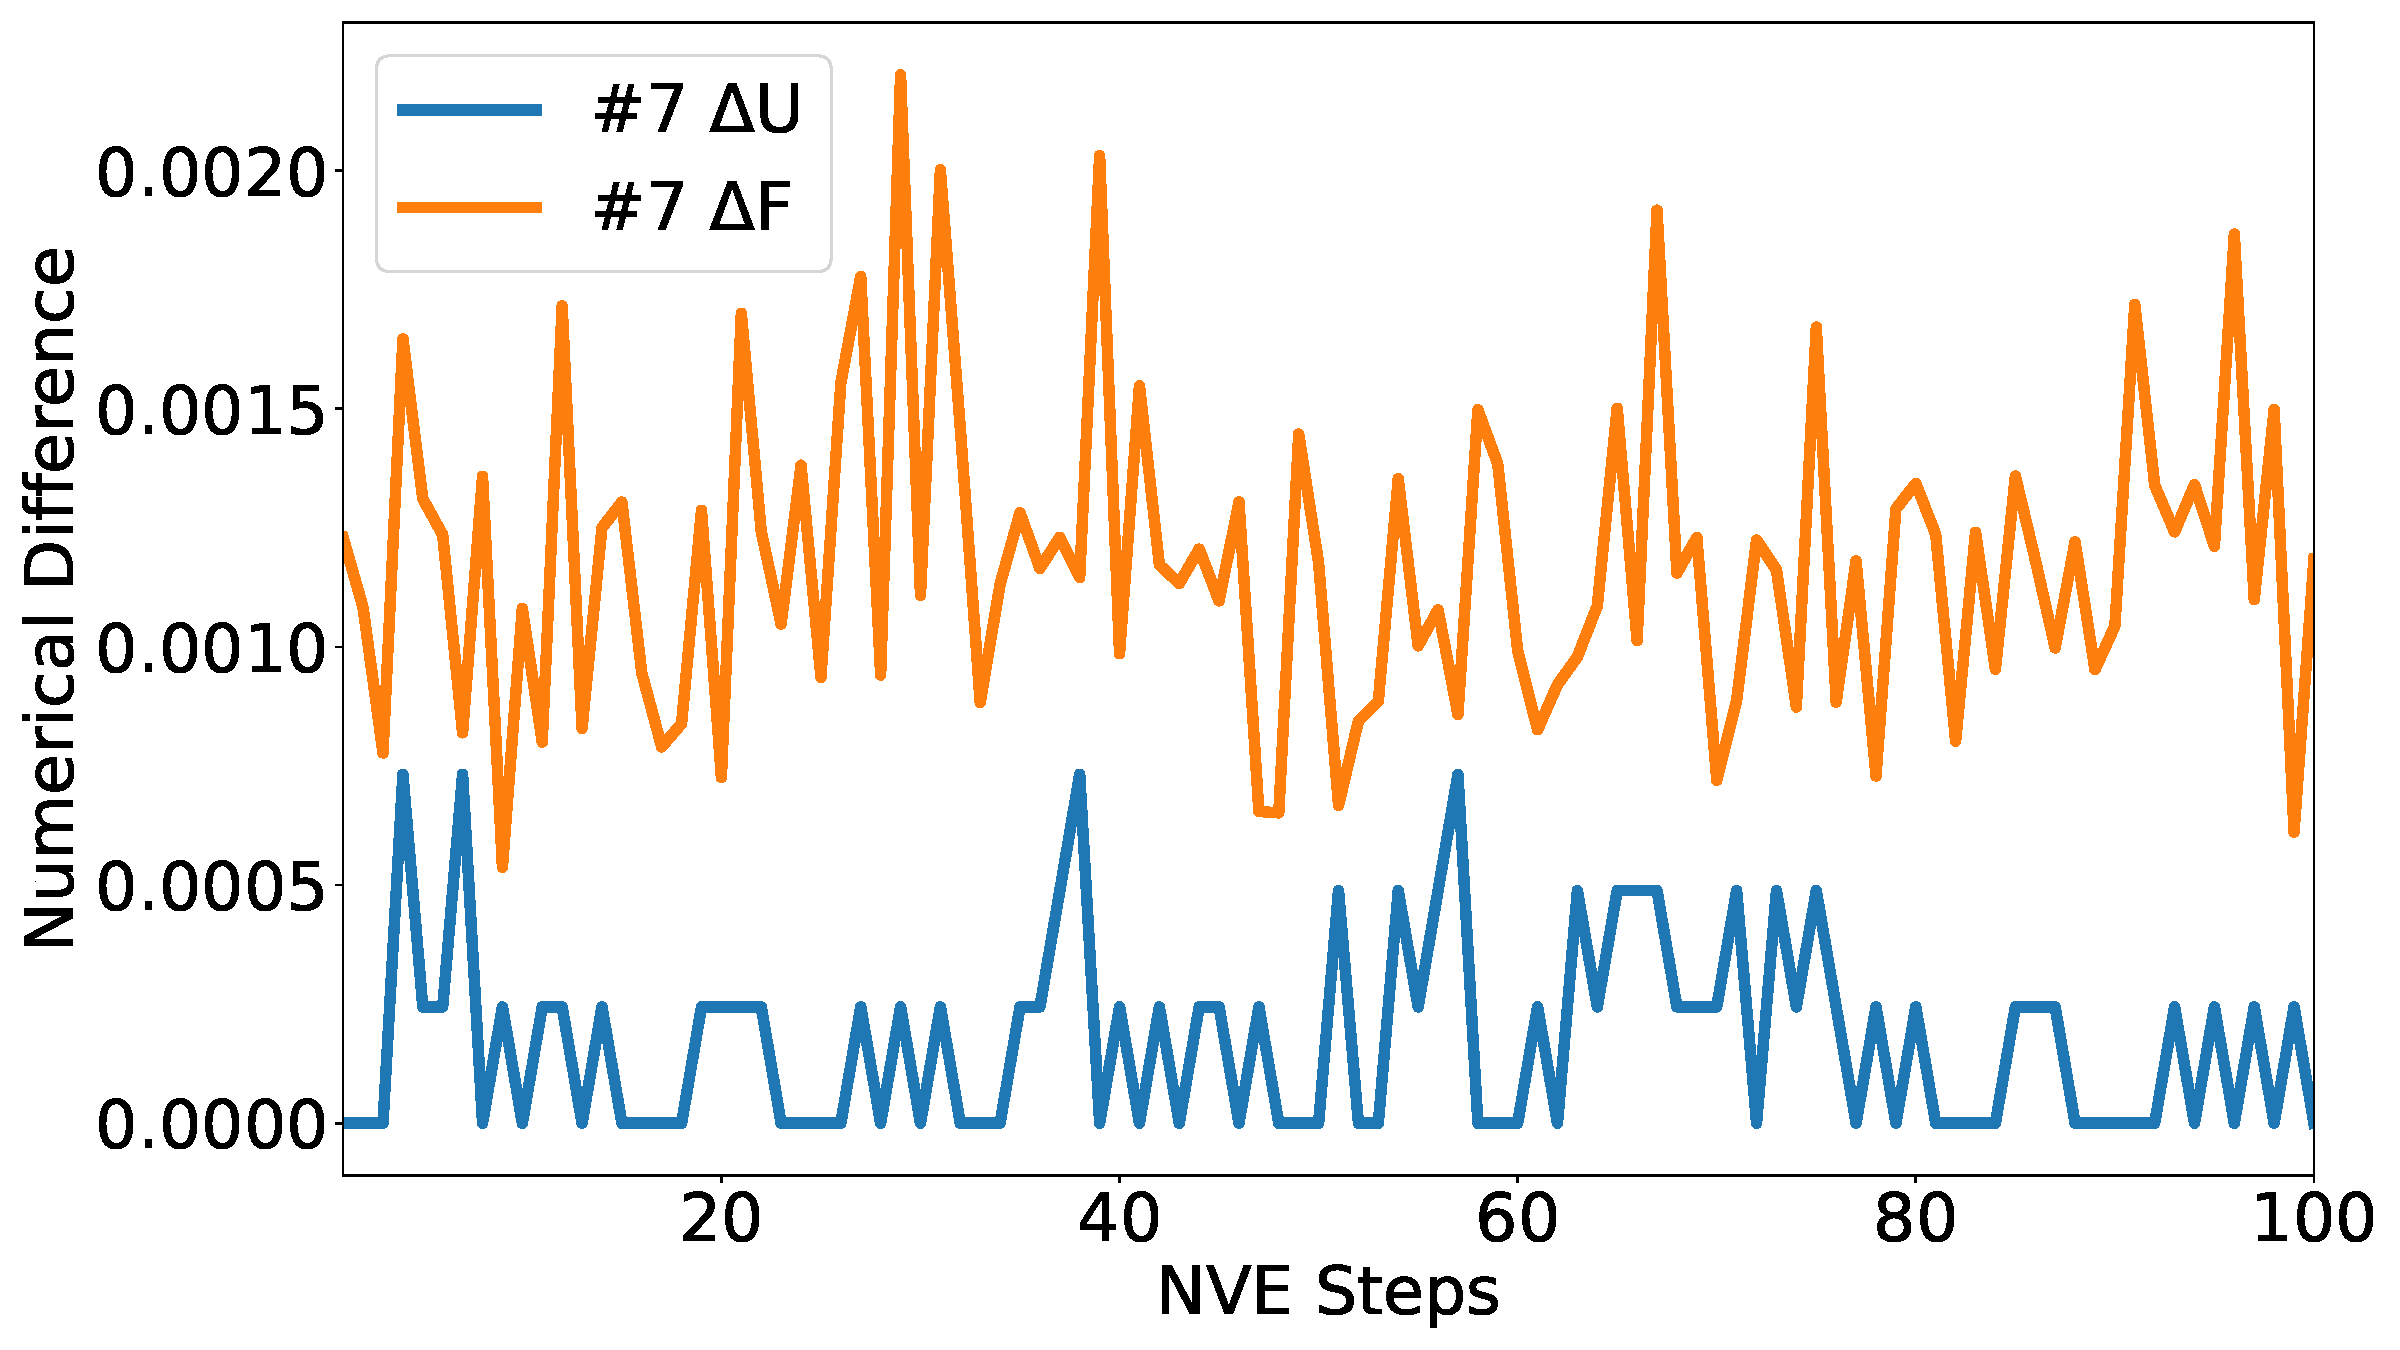
\includegraphics[width=\linewidth]{figs/rerun7.pdf}
\end{subfigure}
\begin{subfigure}{0.48\textwidth}
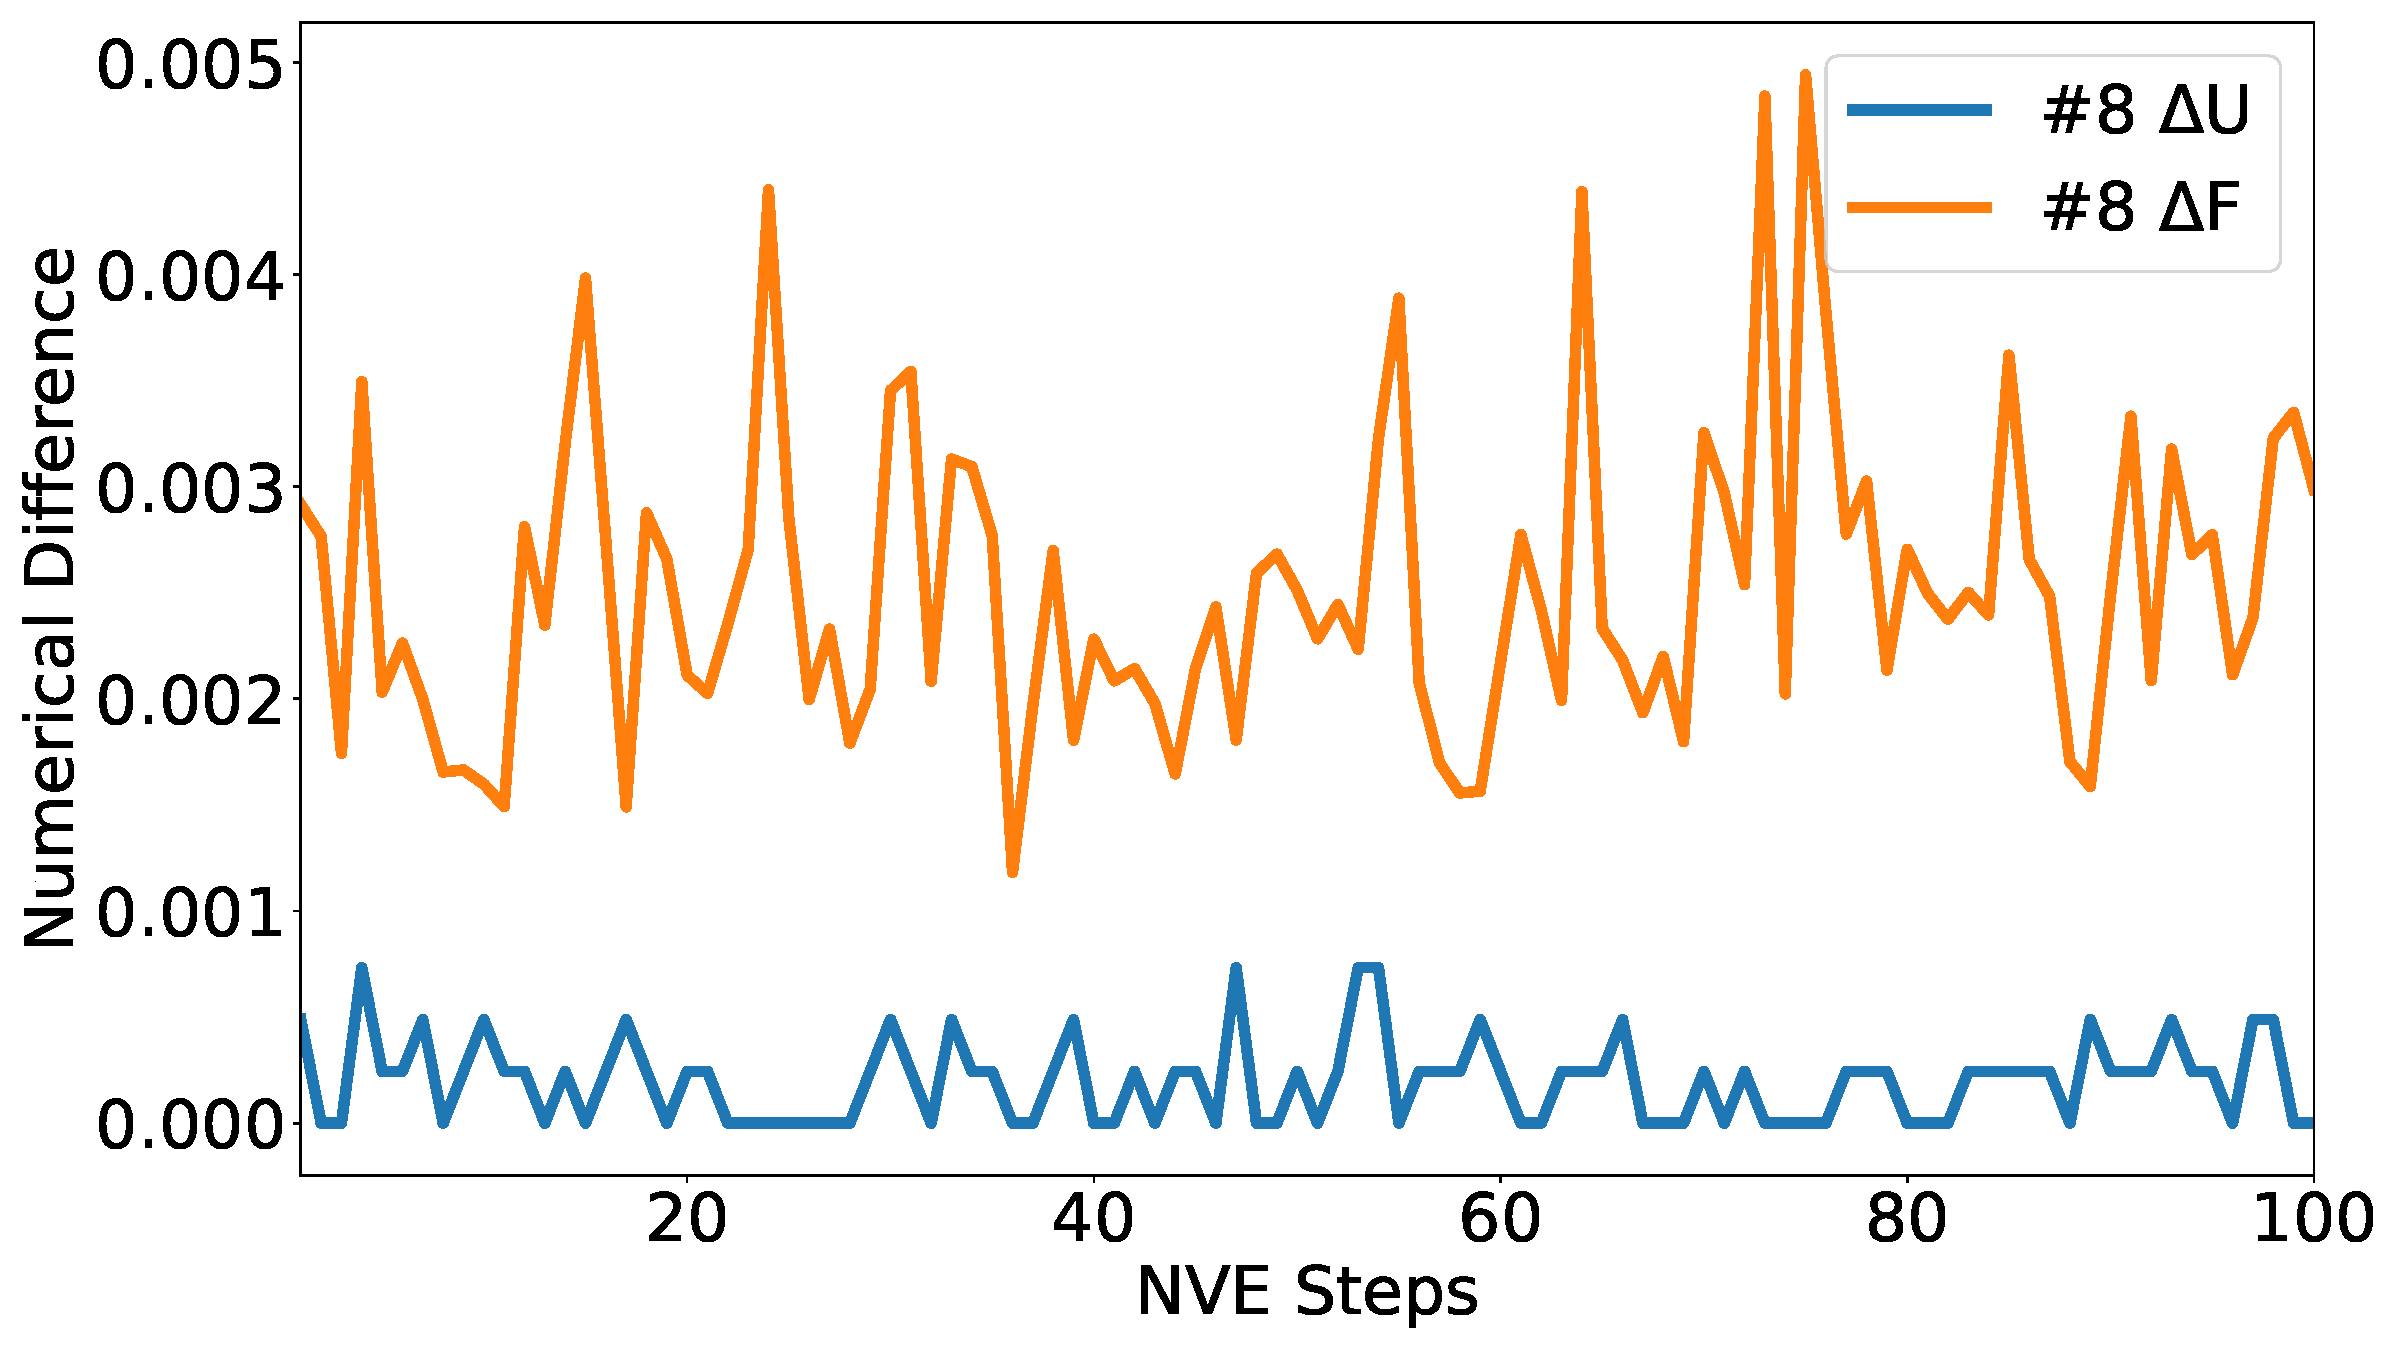
\includegraphics[width=\linewidth]{figs/rerun8.pdf}
\end{subfigure}
\caption{The unsigned differences in potential energies
and root mean square deviation of forces (in kJ/mol and nm)
compared to the baseline,
obtained by recalculating an identical PDB trajectory
across deployment methods.
The number in each subfigure denotes the deployment method
as defined in Table~\ref{tb:deploy8}.}
\label{fig:reruns}
\end{figure*}
